\documentclass[11pt]{article}

\usepackage{amsmath}
\usepackage{tabularx}
\usepackage{subcaption} 
\usepackage{textcomp}
\usepackage{caption}
\usepackage{graphicx}
\usepackage[top=0.8in, bottom=0.8in, left=0.8in, right=0.8in]{geometry}
% Add other packages here %

\usepackage{epstopdf}
\epstopdfDeclareGraphicsRule{.tif}{png}{.png}{convert #1 \OutputFile}
\AppendGraphicsExtensions{.tif}

% Put your group number and names in the author field %
\title{\bf{Classifying Roof Material From Drone Imagery} \\
 An Approach to the Open AI Caribbean Challenge}
\author{Johannes Leonhard Ruether}


% N.B.: The report should not be longer than 3 pages 

\begin{document}
	\maketitle
	
	\section{Introduction (Context and Challenges)}
	
	\subsection{Context}
	
	Regions like the Carribean are regularly hit by rainstorms, floods or earthquakes. Despite being so prone, many houses in those areas are unable to withstand these natural hazards due to poor construction quality. This exposes their inhabitants to a great risk of becoming homeless during the next disaster. 
	
	International programs as the World Bank's Global Program for Resilient Housing are making attempts to retrofit houses to the natural forces they are exposed to. In these large and often informal settlements it is difficult to assess which houses pose especially high risks due to their construction or are damaged and need repair. Exploring these areas on the ground is time consuming and costly. 
	This is why the possibilities of image processing for automatic recognition of vulnerable houses on the basis of drone imagery is explored. Such a technology could assist building inspectors and narrow down large areas to those that are worth a closer inspection on the ground. 
	The material that roofs are made up of is a central indicator of how well a house is prepared against natural disasters. Therefore, classifying roof material from aerial images is a key step to identify precarious houses. \\
	
	\subsection{Open AI Challenge}
	
	The above background led to the initiation of the \textit{Open AI Caribbean Challenge: Mapping Disaster Risk from Aerial Imagery}, which was conducted in between October and December 2020 on \textit{drivendata.org}.	
	This report describes an approach to solve this challenge.\\
	
	\textbf{Probabilities instead of hard labels}
	
	\subsection{Previous Work}
	
	In many applications, the identification of roofs is considered useful. Roof segmentation is often done with LiDAR data, as presented in \cite{Chen2012}. Other papers such as \cite{Soman2019} have successfully attempted roof segmentation using only drone imagery, which is less costly. This step will become relevant for the task at hand. The approach discussed in this report however uses images of roofs that have already been segmented.\\
	
	The identification of roof defects has been addressed in previous works, e.g. \cite{Yudin2018}, in which water stagnation on roofs is measured. Multiple patents such as (e.g. \cite{Shreve2017}) employ aerial images to evaluate damage on individual roofs for insurance purposes. To my best knowledge, academic works on roof material and condition classification from drone imagery on a large scale have not been published. 
	
	\section{Data Description}
	
	\subsection{Images}
	
	The data provided for the challenge consists of high resolution (~4cm) drone imagery of five patches of land: two from Soacha, Colombia, two from Mixco, Guatemala and one from Dennery (St. Lucia).
	For every region, there is one stitched cloud-optimized GeoTIFF file, ranging from 500 to 1800 Megapixels in size.\\

	\begin{center}
		\begin{tabular}{ | m{5cm} | m{10cm}|} 
			\hline
			Platform & WeRobotics (private drone)  \\ 
			\hline
			Source & DrivenData Competition \newline https://www.drivendata.org/competitions/58/disaster-response-roof-type/data/ \\ 
			\hline
			Acquisition Method & Drone Photography  \\ 
			\hline
			SRS  & Ellipsoid (EPSG:32616, 32618, 326120)  \\ 
			\hline
			Spatial/Spectral resolution & 3.8-4.5cm, RGB  \\ 
			\hline
			Type of Product & Cloud-optimized GeoTIFF \\ 
			\hline
		\end{tabular}
	\end{center}
	
	\subsection{Labels}
	
	Roofs are labeled as one of five classes, examples of which are given in Fig.~\ref{fig:mat_examples}: 
	
	\begin{enumerate}
		\itemsep0em
		\item Concrete and Cement: Roofs made out of concrete or cement.
		\item Healthy Metal: Roofs of metal that are intact but may be corrugated or galvanized.
		\item Incomplete: Roofs that are severely damaged or under construction.
		\item Irregular Metal: Roofs that are slightly damaged, rusted or patched.
		\item Other: Roofs that do not fit into other categories (include tiles, red painted, other materials).
	\end{enumerate}

	\begin{figure}
		
		\centering
		\begin{subfigure}[c]{0.32\textwidth}
			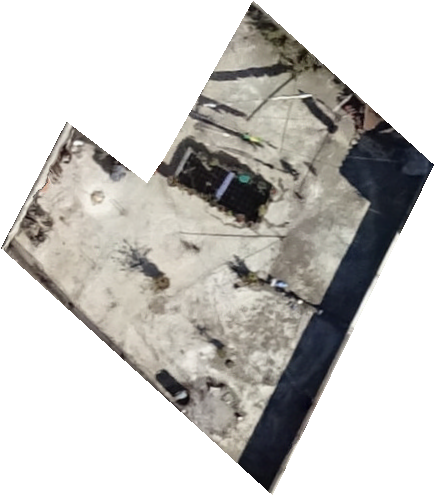
\includegraphics[width=0.47\textwidth]{figures/mat_examples/conc1.png}		
			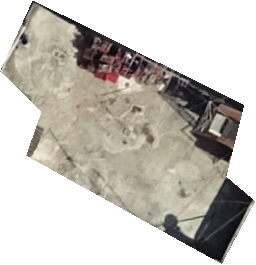
\includegraphics[width=0.47\textwidth]{figures/mat_examples/conc2.png}
			\subcaption{Concrete/Cement}
		\end{subfigure}
		\begin{subfigure}[c]{0.32\textwidth}
			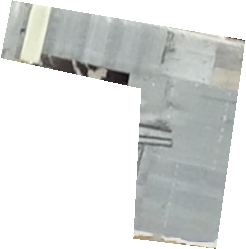
\includegraphics[width=0.47\textwidth]{figures/mat_examples/hm1.png}		
			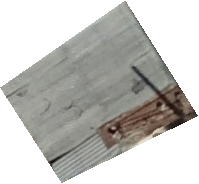
\includegraphics[width=0.47\textwidth]{figures/mat_examples/hm2.png}
			\subcaption{Healthy Metal}
		\end{subfigure}
		\begin{subfigure}[c]{0.32\textwidth}
			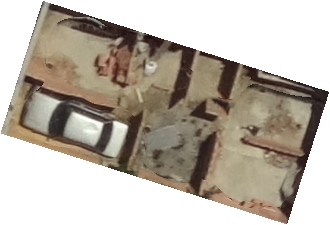
\includegraphics[width=0.47\textwidth]{figures/mat_examples/inc1.png}		
			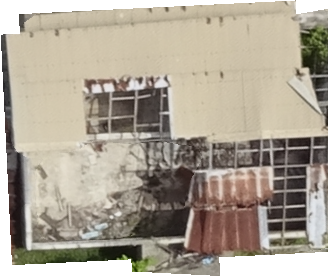
\includegraphics[width=0.47\textwidth]{figures/mat_examples/inc2.png}
			\subcaption{Incomplete}
		\end{subfigure}
		\begin{subfigure}[c]{0.32\textwidth}
			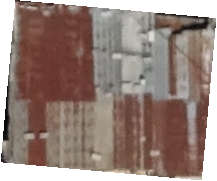
\includegraphics[width=0.32\textwidth]{figures/mat_examples/irr1.png}		
			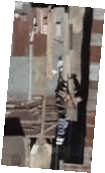
\includegraphics[width=0.32\textwidth]{figures/mat_examples/irr2.png}
			\subcaption{Irregular Metal}
		\end{subfigure}
		\begin{subfigure}[c]{0.32\textwidth}
			\centering
			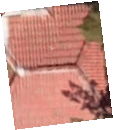
\includegraphics[width=0.35\textwidth]{figures/mat_examples/other1.png}		
			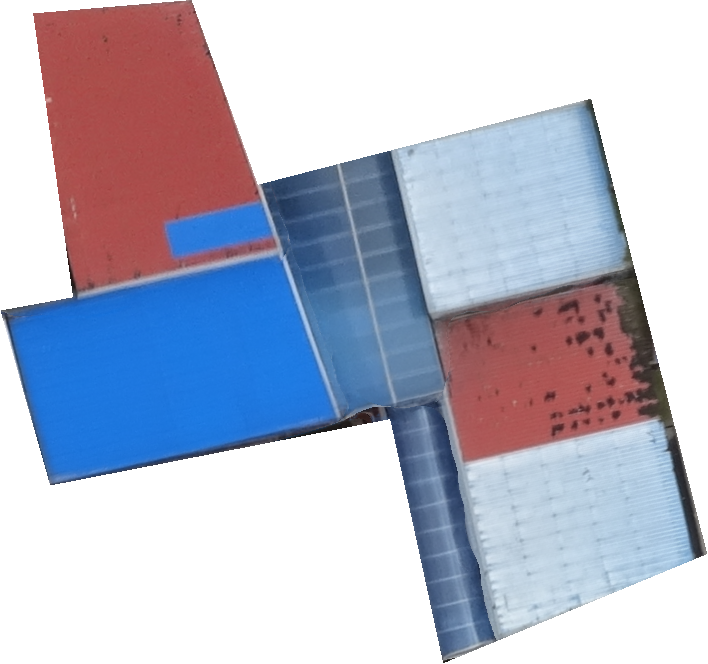
\includegraphics[width=0.45\textwidth]{figures/mat_examples/other2.png}
			\subcaption{Other}
		\end{subfigure}
	\caption{Example images for each material class. (Scales differ)}
	\label{fig:mat_examples}
	\end{figure}

\subsection{Data Noise}

Class membership is unfortunately sometimes ambiguous in the provided groundtruth data. 
First, the labels are used inconsistently. This is especially true for "irregular" and "healthy metal". Where rusty roofs should be labelled as "irregular", many of them get a "healthy metal" label.
Moreover there is confusion about features that make a roof "irregular" or "incomplete".

These inconsistencies might stem from different annotators labeling images.


Second, labels are sometimes clearly incorrect, e.g. concrete roofs are labeled as "healthy metal". Some regions seems to be annotated with more care than others. It is impossible to quantify the extent to which the set is noisy. 
Some examples of these ambiguities are shown in Fig.~\ref{fig:ambiguities}.
The implications for the results are discussed in section~\ref{sec:discussion}.


	\begin{figure}
	
	\centering
	\begin{subfigure}[c]{0.32\textwidth}
		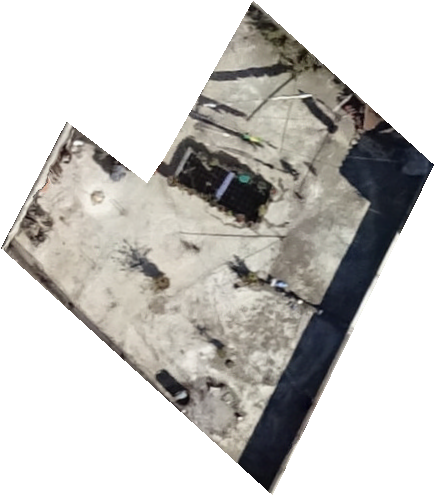
\includegraphics[width=0.47\textwidth]{figures/mat_examples/conc1.png}		
		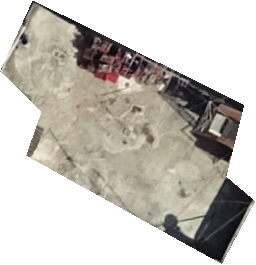
\includegraphics[width=0.47\textwidth]{figures/mat_examples/conc2.png}
		\subcaption{Concrete/Cement}
	\end{subfigure}
	\begin{subfigure}[c]{0.32\textwidth}
		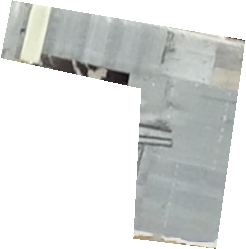
\includegraphics[width=0.47\textwidth]{figures/mat_examples/hm1.png}		
		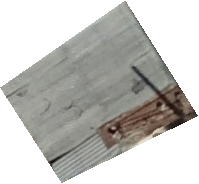
\includegraphics[width=0.47\textwidth]{figures/mat_examples/hm2.png}
		\subcaption{Healthy Metal}
	\end{subfigure}
	\begin{subfigure}[c]{0.32\textwidth}
		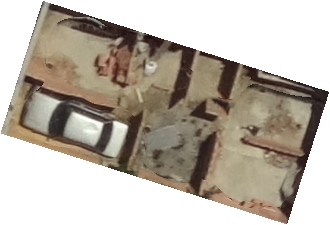
\includegraphics[width=0.47\textwidth]{figures/mat_examples/inc1.png}		
		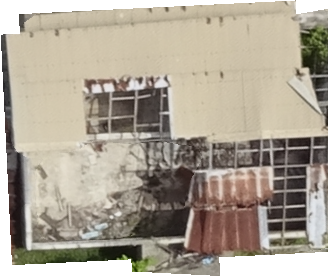
\includegraphics[width=0.47\textwidth]{figures/mat_examples/inc2.png}
		\subcaption{Incomplete}
	\end{subfigure}
	\begin{subfigure}[c]{0.32\textwidth}
		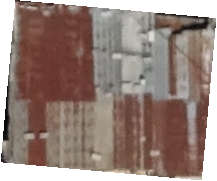
\includegraphics[width=0.32\textwidth]{figures/mat_examples/irr1.png}		
		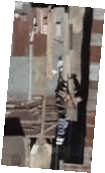
\includegraphics[width=0.32\textwidth]{figures/mat_examples/irr2.png}
		\subcaption{Irregular Metal}
	\end{subfigure}
	\begin{subfigure}[c]{0.32\textwidth}
		\centering
		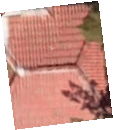
\includegraphics[width=0.35\textwidth]{figures/mat_examples/other1.png}		
		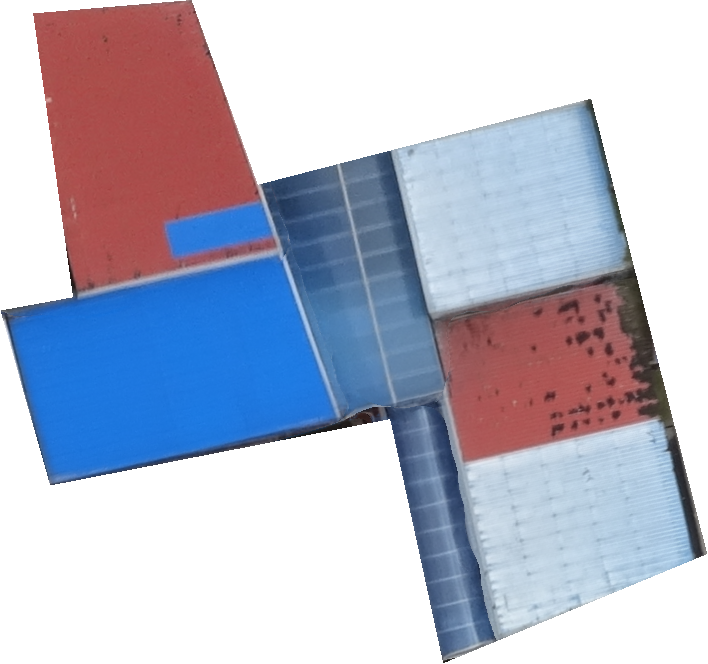
\includegraphics[width=0.45\textwidth]{figures/mat_examples/other2.png}
		\subcaption{Other}
	\end{subfigure}
	\caption{Example images for each material class. (Scales differ)}
	\label{fig:mat_examples}
\end{figure}
	
	\section{Proposed Processing Routine}
	includes flowchart
	
	\section{Results}
	Results qualitative (e.g. maps) and quantitative (e.g. accuracies, statistics). /!\ This implies that you have either access to groundtruth data or digitized/photointerpreted some areas in order to compute accuracies.
	
	\section{Discussion}
	\label{sec:discussion}
	Discussion where you are critical about what has been done and what could be further explored. You have investigated a topic and achieving your initial goal is not always possible in a fixed time frame, however you should be able to assess your situation and what should then be done/improved in order to reach your goal.
	
	
	!!!Noisy Data!!!
	
	\section{Appendix}
	APPENDIX: Include your scripts (Matlab, GoogleEarthEngine or others) and the specific functions you used in QGIS (if applicable)
	*Include a descriptive header on your different scripts
	* Comment your code, use indentation and spacing
	* Only keep the code you used for your latest results
	
	
	
	\bibliography{ipeo} 
	
	\bibliographystyle{ieeetr}

\end{document}